%\newpage
\subsubsection{\stid{3.13} CLOVER Sub-project SLATE}\label{subsubsect:slate}

\paragraph{Overview}

SLATE (Software for Linear Algebra Targeting Exascale)
provides fundamental dense linear algebra capabilities
to the DOE and the HPC community at large.
To this end, SLATE provides
parallel BLAS (basic linear algebra subprograms), norms,
linear system, least squares,
singular value, and eigenvalue solvers.
%
The ultimate objective of SLATE is to replace the
venerable ScaLAPACK (Scalable Linear Algebra PACKage) library,
which has become the industry standard for dense linear algebra operations
in distributed-memory environments, but is past its end of life
and can't be readily retrofitted to support GPUs.
% After two decades of operation,
% ScaLAPACK is past the end of its life cycle and overdue for a replacement,
% as it can hardly be retrofitted to support GPUs,
% which are an integral part of today's HPC hardware infrastructure.

Primarily, SLATE aims to extract the full performance potential and maximum
scalability from modern multi-node HPC machines with
many cores and multiple GPUs per node.
% For typical dense linear algebra workloads, this means getting close
% to the theoretical roofline peak performance and scaling to the full size of
% the machine.
This is accomplished in a portable manner by relying on standards
such as MPI and OpenMP.
%, and encapsulating support for different
% vendors in the BLAS++ and LAPACK++ libraries.
%
% SLATE functionalities will first be delivered to the ECP applications
% that most urgently require SLATE capabilities
% (NWChem, GAMESS, EXAALT, QMCPACK, CANDLE, etc.)
% and to other software libraries
% that rely on underlying dense linear algebra services
% (STRUMPACK, SuperLU, etc.).
Figure~\ref{fig:slate-architecture} shows the role of SLATE
in the ECP software stack.

% While the initial objective of SLATE is to serve as a successful,
% drop-in replacement for ScaLAPACK with support for GPU accelerators,
% the ultimate goal of
SLATE also seeks to deliver dense linear algebra capabilities
beyond the capabilities of ScaLAPACK,
including new features such as communication-avoiding
and randomized algorithms, as well as the potential to
support variable size tiles and block low-rank compressed tiles.

\begin{figure}[htb]
    \centering
    \includegraphics[width=0.75\textwidth]{projects/2.3.3-MathLibs/2.3.3.13-CLOVER/SLATE-architecture.jpg}
    \caption{\label{fig:slate-architecture}
    SLATE in the ECP software stack.}
\end{figure}

\paragraph{Key  Challenges}

\begin{enumerate}

% \item
% \textbf{Designing from the ground up:}
% The SLATE project's primary challenge stems from the need to design the package
% from the ground up, as no existing software package offers
% a viable path forward for efficient support of GPUs
% in a distributed-memory environment.

\item
\textbf{Facing harsh hardware realities:}
SLATE targets a difficult hardware environment, where virtually
all the processing power is on the GPU side.
Achieving efficiency requires aggressive offload to GPU accelerators
and optimization of communication bottlenecks.
% and careful optimization of multiple bottlenecks, including
% interconnect technology lagging behind the computing
% capabilities of the GPUs.

\item
\textbf{Facing harsh software realities:}
SLATE uses cutting-edge software technologies,
including modern C++ features and recent extensions
to the OpenMP standard, which may not be fully supported by compilers
and their runtime environments.
Standardized solutions for GPU acceleration are still in flux.
% Also, while complete parallel programming frameworks exist, at this stage
% they have to be considered research prototypes.

\end{enumerate}

\paragraph{Solution Strategy}

\begin{enumerate}

\item
\textbf{Evolving design:}
Due to the inherent challenges of designing a software package
from the ground up, the SLATE project started
with a careful analysis of the existing and emerging
implementation technologies~\cite{abdelfattah2017roadmap},
followed by an initial design~\cite{kurzak2017designing}
that has solidified~\cite{gates2019slate-design},
but we continue to reevaluate and refactor as needed.

\item
\textbf{Focus on GPUs:}
Efficient GPU acceleration is the primary focus of performance
engineering efforts in SLATE.
Where applicable, highly optimized vendor implementations of GPU operations
are used, such as the batched \texttt{gemm} routine.
Where necessary, custom GPU kernels are developed, as for computing
matrix norms.
Care is taken to hide communication by overlapping it with GPU computations.

\item
\textbf{Community engagement:}
The SLATE team interacts on a regular basis with the OpenMP community,
represented in ECP by the SOLLVE project, and with the MPI community,
represented in ECP by the OMPI-X project and the Exascale MPI project.
The SLATE team also engages the vendor community through our contacts
at HPE Cray, IBM, Intel, NVIDIA, AMD, and ARM.

\end{enumerate}

\paragraph{Recent Progress}

\begin{enumerate}

\item \textbf{Port to AMD and Intel platforms:}
Originally, SLATE was developed using NVIDIA CUDA. We ported BLAS++ to
the AMD ROCm and Intel oneAPI platforms, and use it as a portability
layer for SLATE. Our CUDA kernels were ported to HIP using
AMD's \texttt{hipify} tool. We are also porting kernels to OpenMP
Offload, which provides an option for all platforms (NVIDIA, AMD, and
Intel GPUs).

\item \textbf{Performance improvements:}
We improved performance of several major routines, including
Cholesky, QR, eigenvalue, and singular value decompositions. More components
of Cholesky and QR are now on the GPU. For the eigenvalue
problem, we parallelized a major component and accelerated it using
GPUs, resulting in significant improvements, as shown in
Figure~\ref{fig:slate-he2hb}.

\begin{figure}
    \centering
    \subfloat[][One node]{
        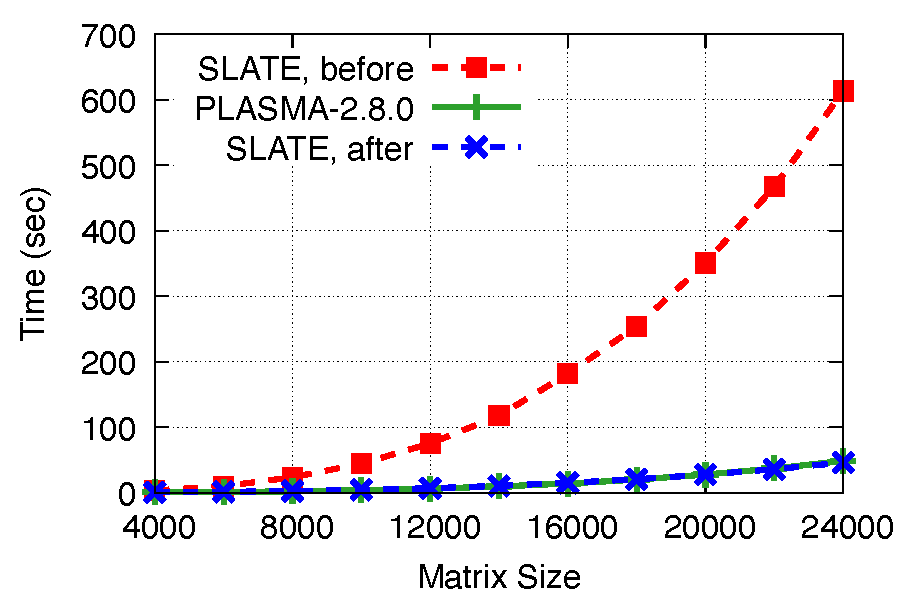
\includegraphics[width=0.4\textwidth]{projects/2.3.3-MathLibs/2.3.3.13-CLOVER/slate-he2hb-1node}
    }
    \subfloat[][Four nodes]{
        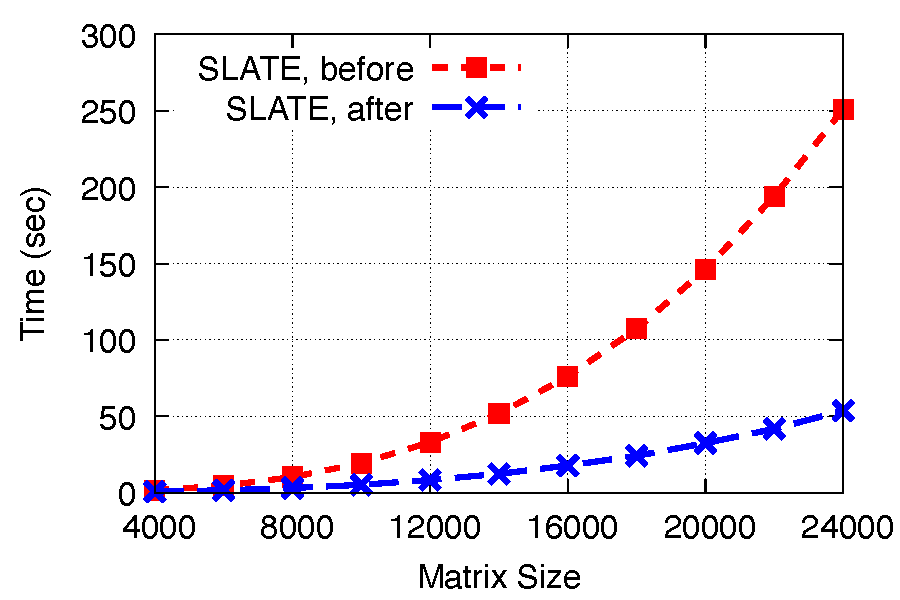
\includegraphics[width=0.4\textwidth]{projects/2.3.3-MathLibs/2.3.3.13-CLOVER/slate-he2hb-4node}
    }
    \caption{Performance improvement in Hermitian reduction to band for
    eigenvalue problem. Each node has $2 \times 10$ core Intel Haswell E5-2650 v3.}
    \label{fig:slate-he2hb}
\end{figure}

\item \textbf{Added eigenvector computation:}
We added computation of eigenvectors to the eigenvalue solver, and are
working on the divide-and-conquer algorithm, which exhibits
better performance than the QR iteration algorithm for computing
eigenvectors.

\end{enumerate}

\noindent
Developments are documented in SLATE Working Notes\footnote{
\url{http://www.icl.utk.edu/publications/series/swans}}.

\paragraph{Next Steps}

\begin{enumerate}

\item \textbf{CA-QR and CA-LU:}
Communication avoiding (CA) routines reorganize the traditional computation
to minimize the number and volume of communications.
Since communication is a major
bottleneck, both between nodes and between different memories within a node,
we expect CA algorithms to improve SLATE's performance.
In particular, we are optimizing QR factorizations with a focus on tall-skinny
matrices, such as solving 10,000,000 $\times$ 1000
least squares problems. There are several avenues to explore including
CA-QR and Cholesky-QR algorithms.

\item \textbf{Optimize Level 2 BLAS:}
For parallel BLAS, the initial implementations focused on the case where
the output matrix $C$ was large. However, the output matrix is often a
single vector, corresponding to Level 2 BLAS, or a few vectors.
For instance, solving a
single right-hand side $b$ in $Ax = b$. These operations require a different
algorithm, so that the computation occurs where the large input matrix $A$
resides, rather than where the output matrix $b$ or $x$ resides. This
lack of Level 2 BLAS optimizations was identified as a major bottleneck
in our mixed-precision iterative refinement algorithms. We will optimize
our existing matrix-multiplication routines to handle these cases,
automatically switching algorithms as needed.

\end{enumerate}
